\section{Devices} Superconducting qubits are composed of an inductor $L$
connected to a capacitor $C$. These are described by the equations of motion of
a harmonic oscillator, with flux $\phi$ through the inductor playing the role of
the canonical position which oscillates out of phase with the charge $Q$ on the
capacitor, this charge playing the part of the canonical momentum
\cite{devoret04_implem_qubit_with_super_integ_circuit}. This LC oscillator has a
resonance frequency that can be specifically engineered as it is given by
$\omega_0 = \nicefrac{1}{\sqrt{LC}}$. The superconducting nature of the
oscillator is of critical importance to maintaining coherence as a superposition
of the ground and first excited states of the LC oscillator decays on a time
scale given by $\nicefrac{1}{RC}$, where $R$ is the resistance. LC circuits, as
macroscopic qubits, are attractive partly because their parameters can be
engineered to whatever values best suit the system in question, but it should be
noted that their size also entail some individuality to each qubit that may lead
to variations in their functioning.

\begin{figure}[h] \centering
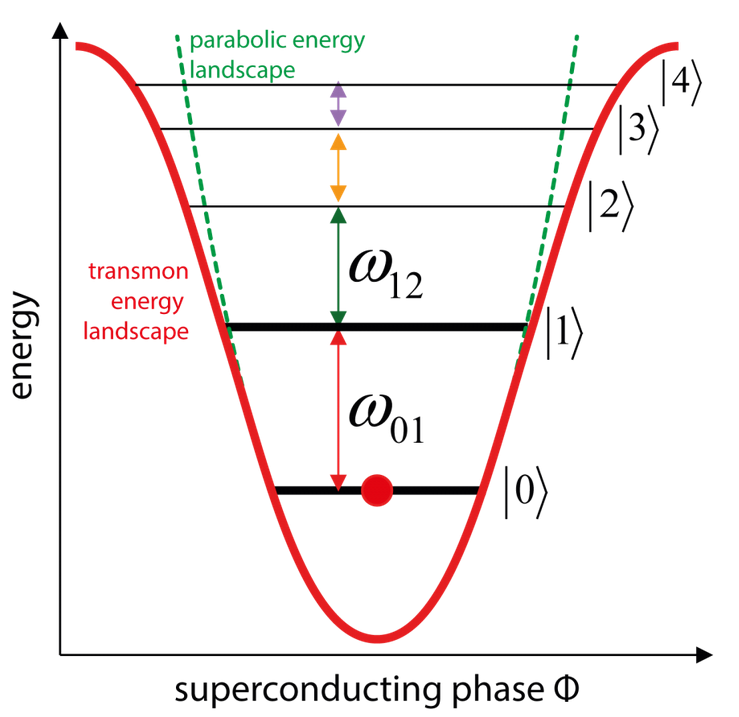
\includegraphics[width=0.48\textwidth]{images/energy_spacing_transmon.png}
  \caption{The energy spacing between levels of an LC oscillator are ordinarily
even, anharmonicity, introduced through the inclusion of a Josephson tunnel
junction, splits the level spacing. Figure from
\cite{dickel20_how_to_make_artif_atoms}.}
  \label{fig:energy_spacing_transmon}
\end{figure}
\newpage
A simple LC circuit alone, though, cannot be an effective qubit. In order to be
able to control the qubit state effectively, the transition frequency between
the states $|0\rangle$ and $|1\rangle$ have to be different enough from all
other transitions, but of course, all transitions between neighbouring states in
the harmonic oscillator potential are the same size. A degree of anharmonicity
is brought in by a Josephson tunnel element with its own non-linear inductance
which is added to the circuit in parallel with the capacitor, make it possible
to individually drive transitions between specific levels in the LC oscillator,
as shown in Fig. \ref{fig:energy_spacing_transmon}. The system's dynamics can
then be effectively confined to just the two lowest energy levels as long as the
driving frequencies for transitions are properly tuned
\cite{devoret04_implem_qubit_with_super_integ_circuit}.

\begin{figure}[h] \centering
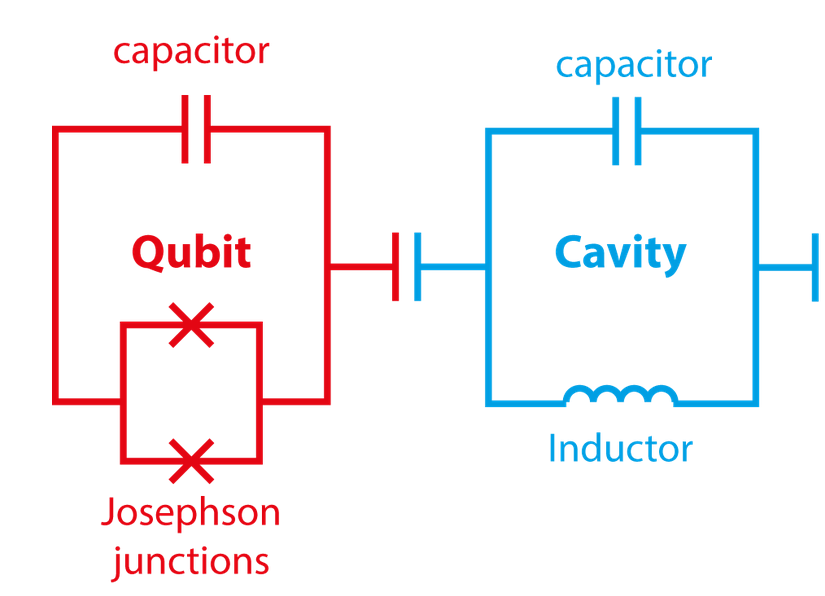
\includegraphics[width=0.48\textwidth]{images/transmon_diagram.png}
  \caption{A schematic of a transmon qubit. The left superconductor maintains
anharmonicity while the right superconductor helps protect it from charge noise.
Figure from \cite{dickel20_how_to_make_artif_atoms}.}
  \label{fig:transmon}
\end{figure}

The devices at the IBM Quantum Experience are transmon qubits. This type of
superconducting charge qubit, shown in Fig. \ref{fig:transmon}, consists of a
qubit circuit coupled to a cavity circuit (a harmonic LC oscillator) which as a
result has a reduced sensitivity to charge noise and has recently shown
coherence times of up to 95$\mu$s and relaxation times of around 70$\mu$s.
\cite{koch07_charg_insen_qubit_desig_deriv,rigetti12_super_qubit_waveg_cavit_with}. Three devices at the IBM Quantum
Experience were chosen to be used in this project. In this section we will
provide an overview of these devices to provide context for the results that
will be discussed below. IBM names its superconducting devices after major
cities, and those we are interested in are code-named Burlington, Melbourne and
Yorktown.

\subsection{Burlington} When comparing the different backends, the first
parameters to take into account in their characterization is the error rates for
single- and two-qubit operations. All three backends use the same universal gate
set, which make their error rates directly comparable. As can be seen in Fig.
\ref{fig:burlington_connections}, this backend has the best gate error rates of
any backend we will consider, with a single-qubit U2 error rate less than
0.065\% for all qubits and a CNOT error rate of less than 1.645\%.

\begin{figure}[h] \centering
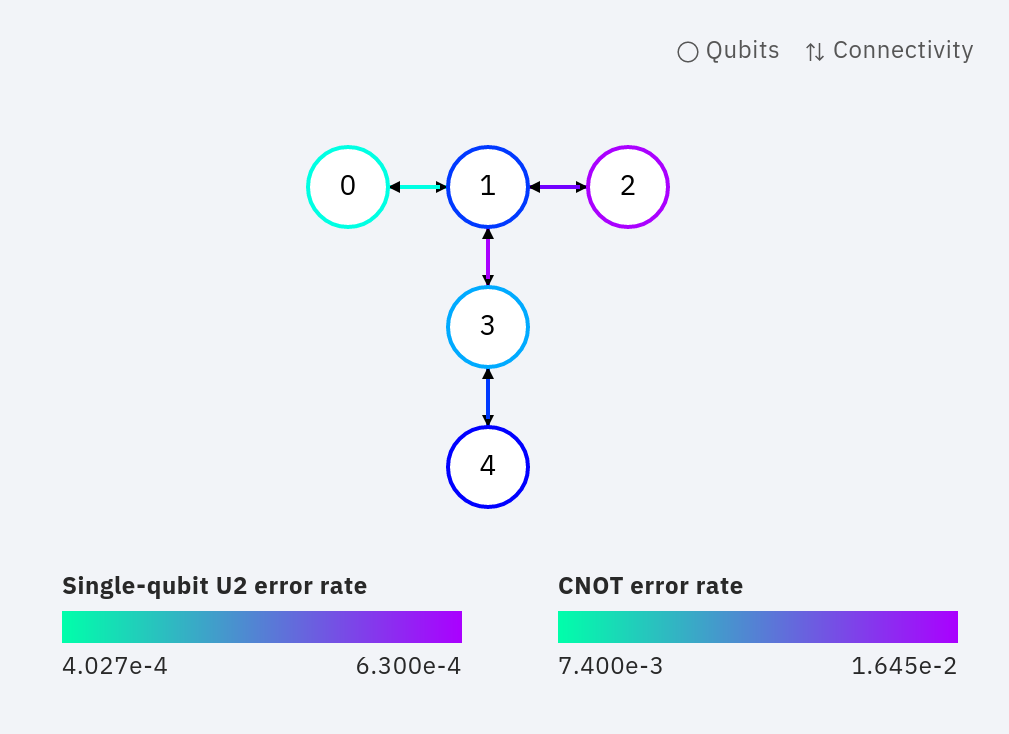
\includegraphics[width=0.48\textwidth]{images/connection_diagram_burlington.png}
  \caption{The T-shaped Burlington device. Though a device with relatively small
error rates, the limited connectivity play a big role in the device's
performance, as many extra gates are needed to implement circuits when there are
few direct connections. Figure from \cite{ibmq_burlington}.}
  \label{fig:burlington_connections}
\end{figure}

In the Melbourne backend (Fig. \ref{fig:melbourne_connections}), single-qubit
gate errors rise to 0.746\%, though the qubits used in all the circuits
implemented here (qubits numbered 0, 1, 2 and 14) all have errors under 0.07\%.
CNOT error between the four qubits of interest to our circuits stays below 4\%.
When choosing which qubits to use for computation, the transpiling program seems
to favour implementation on qubits with the lowest errors (hence the avoidance
of the noisy qubit 13).

The individual character of the qubits is most easily seen in the Melbourne
device. Due to variability in the manufacture of the macroscopic qubits, some
come out noisier than others, and the connections between them likewise suffer
some in-homogeneity.
\begin{figure}[h] \centering
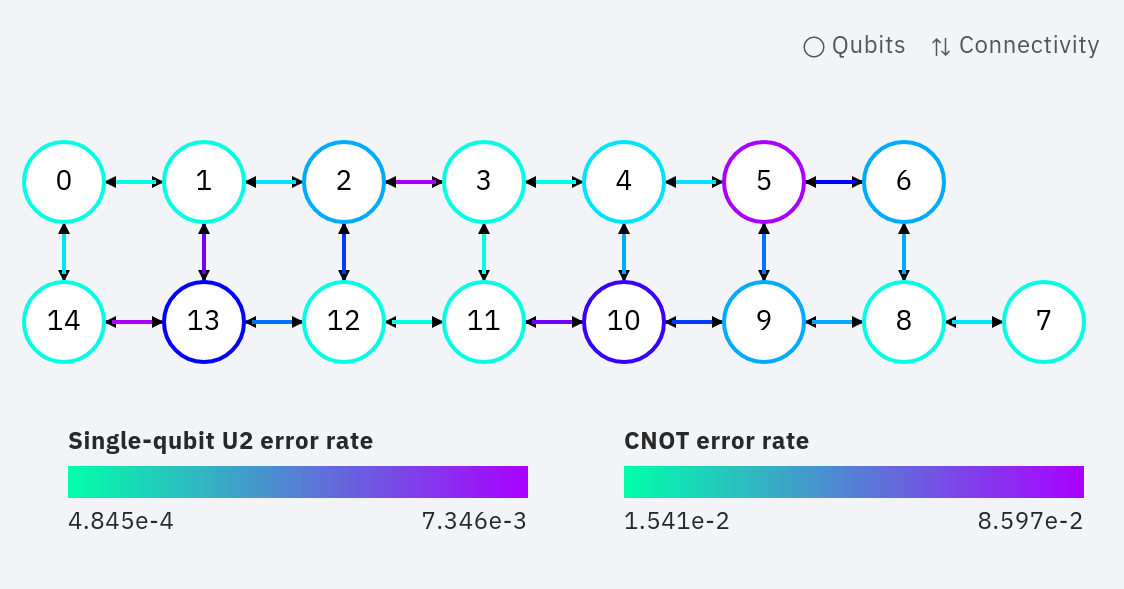
\includegraphics[width=0.48\textwidth]{images/connection_diagram_melbourne.png}
  \caption{The largest publicly available device at IBM Q. The individual
character of the transmons is visible in this diagram through the large
variability in the error rates. Figure from \cite{ibmq_16_melbourne}.}
  \label{fig:melbourne_connections}
\end{figure}

The final backend under consideration, shown in Fig.
\ref{fig:yorktown_connections} comes out between Melbourne and Burlington with
an average single-qubit error rate of 0.05\% and average CNOT error of 2.276\%.
However, as we will see in the results, these gate error rates are far from the
whole story when it comes to explaining the performance of various backends.
\begin{figure}[h] \centering
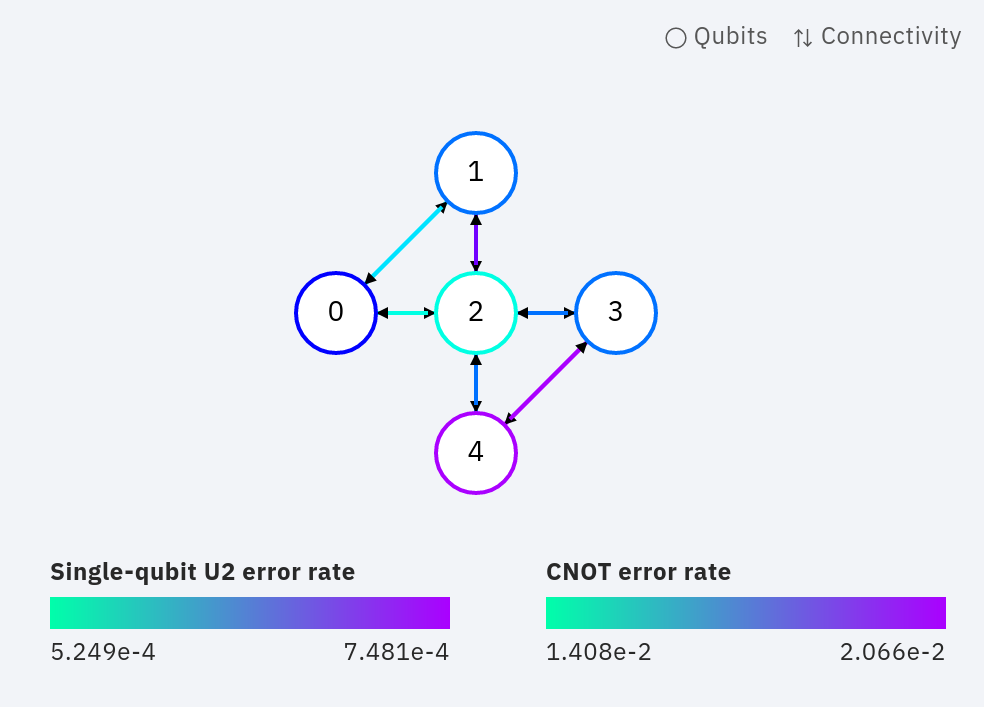
\includegraphics[width=0.48\textwidth]{images/connection_diagram_ibmqx2.png}
  \caption{The most densely connected 5-qubit device at IBM Q. As we will see,
equally as important as the single-qubit and CNOT error rates is the degree of
connectivity in a device. Figure from \cite{ibmq_yorktown}.}
  \label{fig:yorktown_connections}
\end{figure}
\newpage
\begin{table} \centering
	\begin{tabular}{lrrrr} \toprule Backend & $U_2 (\%)$ & $CNOT (\%)$ \\ \midrule
		Burlington & 0.050 & 1.213 \\ Melbourne & 1.258 & 2.156 \\ Yorktown & 0.689 &
		2.275 \\ \bottomrule
	\end{tabular}
	\caption{Average percent error on single-qubit $U_2$ gates and CNOT gates for
		the three devices used to implement the circuits of interest. All averages taken
		from data provided at \cite{ibmq_burlington,ibmq_16_melbourne,ibmq_yorktown}.}
	\label{tb:average_errors}
\end{table}
One consideration that is not reflected in the gate error rates which has a
significant impact on the fidelity of the outputs of circuits is the number of
direct connections between qubits. Burlington may have the lowest average error
rates for gate operations of all the three devices (shown in Table
\ref{tb:average_errors}), but as we will show, this doesn't translate to better
output fidelities in every case. In fact, because the number of gates required
to implement each circuit will vary from device to device, the optimal backend
on which to conduct a given computation will ultimately depend more on the
configuration of each backend, rather than gate errors.

%%% Local Variables:
%%% mode: latex
%%% TeX-master: "report"
%%% End: